\section{Адаптивный алгоритм распределения заказов}

	\subsection{Описание}

		В данном Приложении описывается стратегия поиска подходящего водителя под срочные городские заказы. О поиске водителя под предварительные и портовые заказы, а также описание работы робота в режимах “поиск по адресу” и “хочу домой” смотреть в соответствующих разделах ТЗ.

		В критической ситуации, когда новые заказы поступают быстрее, чем водители успевают их выполнять, алгоритм из SRV-9.2.1 может давать много отказов (когда нет свободной машины) и опозданий ко времени подачи. Причина этого в том, что на каждый заказ он подбирает “локально оптимального водителя” - того, что ближе к данному клиенту, и при этом игнорирует требования других заказов, находящихся в данный момент в системе.

		В качестве альтернативы можно предложить алгоритм на основе методов математического программирования, который осуществляет глобальную оптимизацию, учитывая требования одновременно всех заказов, ожидающих обслуживания водителями. Основная его идея - назначить “плохого” (не ближайшего) водителя на заказ с более поздним временем подачи, чтобы тем временем отправить более близкого водителя на появившийся неподалеку от него более срочный заказ (и в результате успеть выполнить оба). При этом неизбежно потребуется возможность несколько раз менять назначенного на заказ водителя (это будет происходить при появлении новых заказов), пока по нему еще не пришло время ехать к клиенту.

	\subsection{Термины}

		\begin{table}[htb]
	        \begin{center}
	        \caption{Термины}
	        \label{appendices_termins}
	        \setlength{\extrarowheight}{2mm}
	        \begin{tabular}{|p{6cm}|p{9cm}|}
	           
	           \hline Предварительное назначение & Назначение заказа на водителя с включенным роботом, которое, пока водитель не выехал к клиенту, может быть изменено.\\ [2mm]

	           \hline Матрица & Таблица, в которой для каждого из заказов в состоянии “предварительно назначен” хранится время подачи по нему машины каждым из водителей (рассматриваются только, те, кто подходит по параметрам и попадает в диапазон).\\ [2mm]

	           \hline Резерв времени & Время, которое останется в запасе у данного водителя, если он немедленно примет данный заказ и приедет к месту подачи машины (закончив текущий заказ, если такой имеется).\\ [2mm]

	           \hline Расчетное время подачи & Время, через которое данный водитель сможет подать машину по данному заказу, если он немедленно примет этот заказ (закончив текущий заказ, если такой имеется).\\ [2mm]

	           \hline Доступный водитель & Водитель, который либо “свободен”, либо “в пути” с включенным роботом.\\ [2mm]    

	           \hline
	        \end{tabular}
	        \end{center}
      	\end{table}

    \subsection{Пример}

    	Допустим в диспетчерскую поступило два заказа - Z1 и Z2, и поблизости от них есть два свободных водителя с включенным роботом - В1 и В2.

    	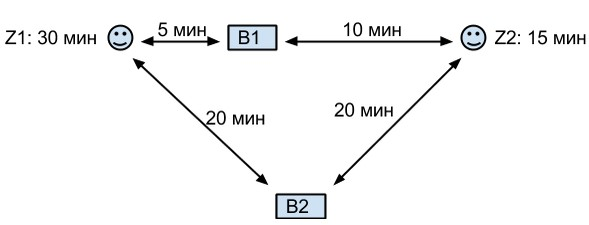
\includegraphics{images/appendices/appendix_example}

    	Заказ Z2 более срочный - 15 минут до подачи машины, Z1 менее срочный - 30 минут.

		В1 может за 5 минут доехать до клиента Z1 и за 10 минут - до клиента Z2 (т.е. к менее срочному заказу ему ехать быстрее).

		Водитель В2 едет до обоих заказов по 20 минут. Т.е. выполнить заказ Z2 без опоздания он не может в принципе.

		Это представлено в таблице:

		\begin{table}[htb]
	        \begin{center}
	        \caption{Пример}
	        \label{appendices_example_table}
	        \setlength{\extrarowheight}{2mm}
	        \begin{tabular}{|p{2cm}|p{2cm}|p{2cm}|}
	           \hline   \textbf{ }&\textbf{Z1}&\textbf{Z2} \\ [2mm]

	           \hline B1 & 5 мин & 10 мин\\ [2mm]

	           \hline B2 & 20 мин & 20 мин\\ [2mm]    

	           \hline
	        \end{tabular}
	        \end{center}
      	\end{table}

      	\textbf{Рассмотрим ситуацию, когда заказ Z1 (30 мин) поступил в диспетчерскую раньше, чем Z2.}

		\textbf{“Плохой” алгоритм}

		В соответствии с описанным выше алгоритмом, назначение водителей будет происходить следующим образом:
		\begin{enumerate}

			\item{На заказ Z1(30 мин) будет назначен ближайший к нему водитель В1. Он 20-25 минут будет отдыхать, после чего поедет выполнять этот заказ.}

			\item{При поступлении заказа Z2(15 мин) водитель В1 будет уже занят и диспетчеру придется согласовывать с клиентом \textbf{5-минутное опоздание}, после чего за ним поедет водитель В2. В это время водитель В1 “отдыхает” перед выполнением заказа Z1, который до этого был за ним закреплен.}

		\end{enumerate}

		\textbf{“Хороший” алгоритм}

		Чтобы решить эту проблему, нам потребуется возможность менять назначенного на заказ водителя, если тот еще не поехал этот заказ выполнять:
		\begin{enumerate}

			\item{Поступивший первым заказ Z1(30 мин) будет добавлен в список “текущих заказов” и “предварительно назначен” на водителя В1 (ближайшего к нему).}

			\item{При поступлении заказа Z2(15 мин) он также будет добавлен в список “текущих заказов”, после чего произойдет перерасчет всех назначений с целью минимизации опозданий. При этом водитель В1 будет снят со “старого” заказа Z1(30 мин) и назначен на новый, более срочный, заказ Z2(15 мин) (по которому сможет подать машину в течение 5 мин). Оставшийся без водителя заказ Z1(30 мин) уйдет водителю В2, который за 20 минут успешно доедет до этого клиента.}

			\item{При выезде к клиенту оба водителя перейдут в состояние “едет к клиенту”, после чего система уже не сможет назначить им никакой другой пришедший позже заказ.}

		\end{enumerate}

	\subsection{Диаграммы состояний}

		Для реализации описанного подхода нам потребуется ввести новое состояние заказа - “предварительно назначен”. Расширенные диаграммы состояний водителя и заказа показаны ниже.

		\subsubsection{Состояния водителей}

			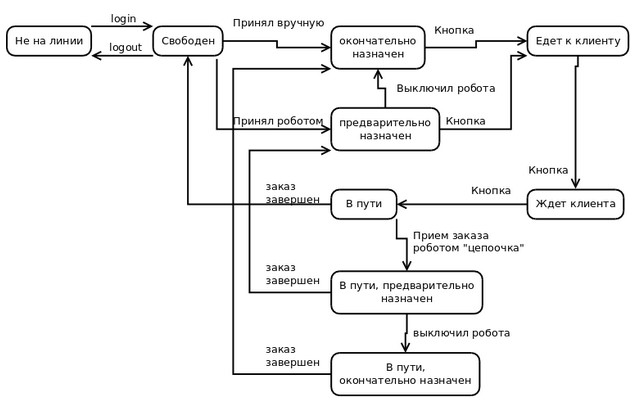
\includegraphics{images/appendices/drivers_state}

			Примечание: пока водитель находится в состоянии “предварительно назначен”, на него могут многократно назначаться новые заказы (с перенесением старых на других водителей). Подтверждение водителя, что он “в курсе” требуется только при первом назначении.

		\subsubsection{Состояния заказов}

			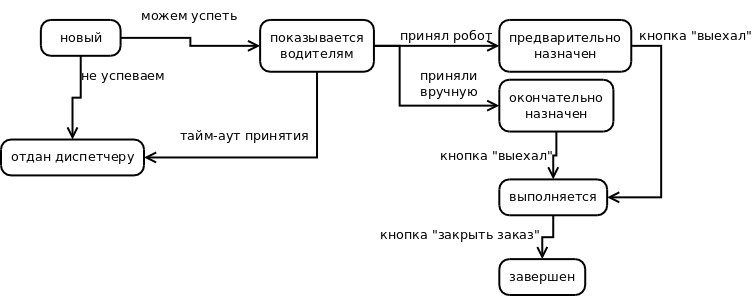
\includegraphics{images/appendices/orders_state}

			Примечание: пока заказ находится в состоянии “предварительно назначен”, он может быть многократно переназначен на другого водителя (это происходит по мере поступления новых заказов, которые невозможно выполнить вовремя при сохранении старых назначений).

	\subsection{Описание алгоритма}

		В условиях высокой интенсивности поступления заказов наша основная задача - не опаздывать ко времени подачи.  Поэтому основная величина, которая нас будет интересовать по каждой паре “заказ+водитель” - это резерв времени: сколько времени останется у данного водителя в резерве, если он без промедления поедет выполнять данный заказ. Например, в примере выше, если водитель В1 поедет выполнять заказ Z2(30 мин), то он за 5 минут до него доедет, и в резерве у него останется 25 минут.

		Таблица с резервами времени:

		\begin{table}[htb]
	        \begin{center}
	        \caption{Резервы времени}
	        \label{appendices_algorithm_expl}
	        \setlength{\extrarowheight}{2mm}
	        \begin{tabular}{|p{2cm}|p{2cm}|p{2cm}|}
	           \hline   \textbf{ }&\textbf{Z1}&\textbf{Z2} \\ [2mm]

	           \hline B1 & 25 мин & 5 мин\\ [2mm]

	           \hline B2 & 10 мин & -5 мин\\ [2mm]    

	           \hline
	        \end{tabular}
	        \end{center}
      	\end{table}

      	Число -5 для пары В2+Z2 означает, что в этом случае произойдет опоздание.

    \subsection{Матрица}

    	Для реализации упомянутого выше “хорошего” алгоритма, сервер хранит в памяти матрицу, аналогичную приведенной только что. На основании нее при каждом поступлении нового заказа заново производит назначение водителей. Когда водитель приступает к выполнению заказа - т.е. выезжает к клиенту - данный заказ удаляется из матрицы и в последующих переназначениях не участвует.

    	\subsubsection{Пересчет матрицы}

    		\begin{itemize}
    			\item{Когда водитель приступает к выполнению заказа (“еду к клиенту”), а также при его удалении - из матрицы удаляется соответствующий столбец, а также все строки, в которых все элементы равны “минус бесконечности”.}

    			\item{При добавлении заказа - в матрицу добавляется этот заказ (столбец) и N водителей с наибольшим резервом времени по данному заказу (при условии, что они подходят по параметрам и диапазону взятия заказа). Для всех уже присутствовавших в матрице водителей вычисляются и заносятся в матрицу их “резервы времени” по новому заказу. N задает администратор, для начала положим N=100.}

    			\item{При других изменениях в системе (перемещение по карте свободных водителей, вход и выход водителей из системы, изменение настроек робота и др.) производится коррекция элементов матрицы.}
    		\end{itemize}

    	\subsubsection{Пересчет предварительных назначений}

    		Основная идея минимизации опозданий - это решение для нашей матрицы \href{https://ru.wikipedia.org/wiki/%D0%9B%D0%B8%D0%BD%D0%B5%D0%B9%D0%BD%D0%B0%D1%8F_%D0%B7%D0%B0%D0%B4%D0%B0%D1%87%D0%B0_%D0%BE_%D0%BD%D0%B0%D0%B7%D0%BD%D0%B0%D1%87%D0%B5%D0%BD%D0%B8%D1%8F%D1%85_%D0%B2_%D1%83%D0%B7%D0%BA%D0%B8%D1%85_%D0%BC%D0%B5%D1%81%D1%82%D0%B0%D1%85}{задачи о назначениях в узких местах} (linear bottleneck assignment problem, LBAP) с целью \textit{максимизации минимального резерва времени}. Или - что то же самое - минимизации максимального опоздания.

			Эта задача решается повторно каждый раз, когда при поступлении нового заказа для него не находится доступного водителя, который успел бы подать машину вовремя. Так как такой пересчет изменят установленные ранее предварительные назначения, то нам нужно следить за тем, чтобы не “испортить” ни одно из них (т.е. не получить отрицательный резерв времени), а также при необходимости оповещать об изменении назначений водителей.

			Конкретные действия при поступлении нового заказа:

			\begin{enumerate}
				\item{Выбор лучших N водителей для данного заказа, расчет для них резервов времени по этому заказу и добавление этой информации в матрицу (см. выше “пересчет матрицы”).}

				\item{Поиск водителя с наибольшим резервом времени по данному заказу среди тех, кому еще не произведено предварительное назначение какого-либо заказа.}

				\item{Если этот резерв времени больше нуля - т.е. водитель успевает подать машину вовремя - то заказ отсылается водителю и может быть принят им в течение 30 секунд (водитель с роботом примет его сразу). Принятый заказ \textit{предварительно закрепляется} за данным водителем.}

				\item{Если водитель отказался - его \textit{резерв времени} по данному заказу (в матрице) приравнивается к “минус бесконечности” и повторяется шаг. №2.}

				\item{Если водитель принял заказ вручную - без робота - то заказ окончательно закрепляется за данным водителем и удаляется из матрицы.}

				\item{\textbf{Если не нашлось подходящего водителя с резервом времени, большим нуля, происходит решение \textit{задачи о назначениях в узких местах стандартным} “пороговым” алгоритмом. Результат этого решения - новый набор предварительных назначений водителей на уже имеющиеся заказы.}}

				\item{Если это не позволило получить решение без опозданий - сообщение диспетчеру.}

				\item{Если позволило - соответствующие водители оповещаются об изменении заказа. У всех них включен робот, поэтому отказаться они не могут (30 сек на подтверждение, если водитель не в пути; а водители “в пути” узнают подробности заказа, когда приедут).}

				\item{Если кто-то из водителей не реагирует на изменение заказа - окончательно закрепляем за ним его предыдущий заказ, удаляем этот заказ из матрицы и повторяем процедуру с шага №6.}

				\item{В результате получаем новый набор назначений \textit{без опозданий}. Чтобы при добавлении следующего заказа не “испортить” присутствующие в данный момент в матрице заказы (т.е. чтобы при следующем пересчете не назначить на них опаздывающих водителей) - заменяем все отрицательные элементы матрицы на “минус бесконечность”.}
			\end{enumerate}

	\subsection{Заключительные замечания}

		Как видим, “борьба за заказы” не обходится даром: предложенный алгоритм предъявляет дополнительные требования как к водителям, так и к диспетчерам:

		\begin{enumerate}
			\item{Работает только тогда, когда большинство водителей ездит с включенным роботом в режиме “цепочка”.}

			\item{Непривычен для диспетчеров, т.к. до последнего момента оттягивает окончательное закрепление водителя за заказом, и пока водитель не выедет к клиенту, заказ может несколько раз “перескакивать” на других водителей.}
		\end{enumerate}

		При этом алгоритм осуществляет глобальную оптимизацию, учитывая при назначении водителей потребности сразу нескольких заказов одновременно. Это позволяет назначить на менее срочный заказ более отдаленную машину, “пожертвовав” более близкую машину на выполнение другого, более срочного заказа. В итоге, если это действительно будет работать в конкретных условиях рынка автоперевозок Москвы - получим меньше опоздания и больше выполненных заказов.

		Безусловно, при реализации и тестировании, многое из вышеизложенного нужно будет изменить. И в итоге это может вообще не заработать. Однако, опыт других организаций (см. список литературы) показывает, что внедрение “интеллектуальных” систем назначения заказов на водителей позволяет увеличить эффективность использования машин на 5-10\%. Правда, лучше всего это работает, когда организация имеет максимальный контроль над своими водителями: водитель едет туда, куда ему скажет система, и собственных решений не принимает. В нашем случае это не всегда так.

	\subsection{Литература}

		\begin{enumerate}
			\item{Glaschenko, A.; Ivaschenko, A.; Rzevski, G. \& Skobelev, P. (2009), 'Multi-Agent Real Time Scheduling System for Taxi Companies':\\ \url{http://www.rzevski.net/09%20Scheduler%20for%20Taxis.pdf}}

			\item{Сонькин Д. М. АДАПТИВНЫЙ АЛГОРИТМ РАСПРЕДЕЛЕНИЯ ЗАКАЗОВ НА ОБСЛУЖИВАНИЕ АВТОМОБИЛЯМИ ТАКСИ // Известия ТПУ. 2009.  №5. URL:\\ \url{http://cyberleninka.ru/article/n/adaptivnyy-algoritm-raspredeleniya-zakazov-na-obsluzhivanie-avtomobilyami-taksi}}
		\end{enumerate}